% Как посчитать eigenvalues через QR и еще как-то вычислительно эффективно?

\ProvidesFile{section_5_diagonal}[Section 5]

\newpage

\section{Eigenvalues and Where to Find Them}

\subsection{Motivation for eigenvalues and eigenvectors}

%TODO
%* Круги Гершгорина (есть в Гилберте Стрэнге и в Акслере, стр.170).

\begin{example}\label{kitten_transform}
Question 1: What is the geometric meaning of the linear operator with matrix
$$
A = \begin{pmatrix}
    2 & 0 \\
    0 & -2
\end{pmatrix}?
$$
See the figures:
\begin{center}
    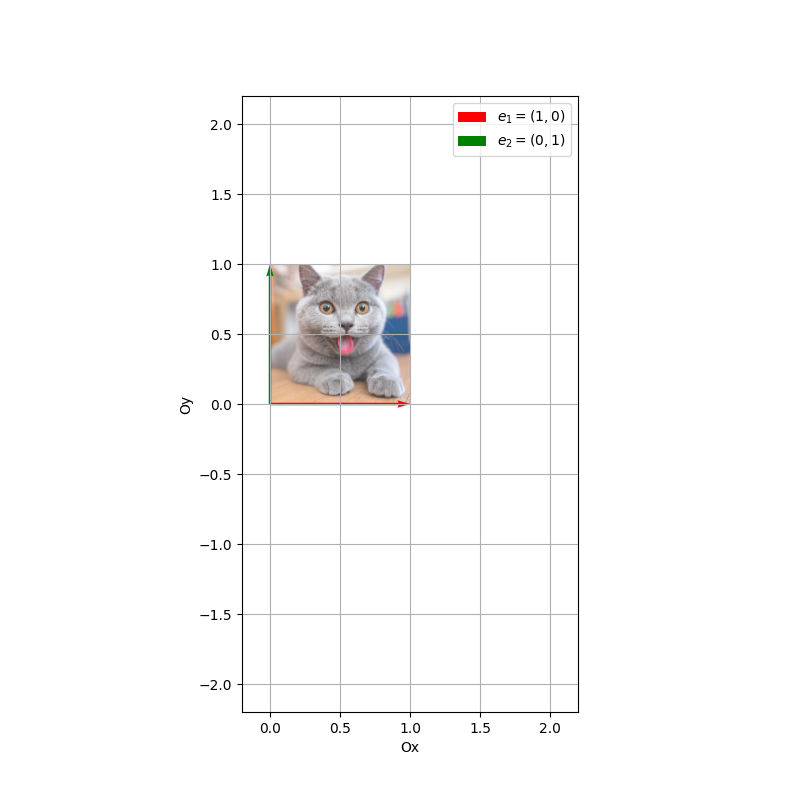
\includegraphics[width=0.45\textwidth]{Images/cat_plot_1.png}
    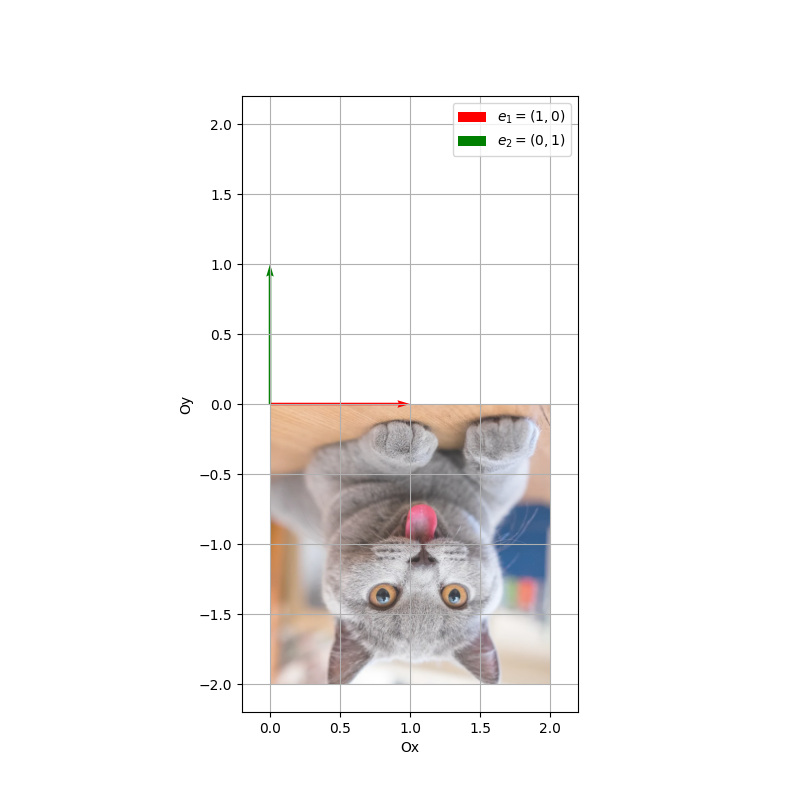
\includegraphics[width=0.45\textwidth]{Images/cat_plot_2.png}
\end{center}

Question 2: What is the geometric meaning of the linear operator with matrix 
$$
B = \begin{pmatrix}
    \frac{2}{3} & -\frac{8}{3} \\
    -\frac{4}{3} & -\frac{2}{3}
\end{pmatrix}?
$$
It turns out that after a change of basis we obtain the following relation:
$$
B^{\prime} = \begin{pmatrix}
    2 & 0 \\
    0 & -2
\end{pmatrix} =
\begin{pmatrix}
    \frac{2}{3} & \frac{1}{3} \\
    -\frac{1}{3} & \frac{1}{3}
\end{pmatrix}^{-1}
\begin{pmatrix}
    \frac{2}{3} & -\frac{8}{3} \\
    -\frac{4}{3} & -\frac{2}{3}
\end{pmatrix}
\begin{pmatrix}
    \frac{2}{3} & \frac{1}{3} \\
    -\frac{1}{3} & \frac{1}{3}
\end{pmatrix}.
$$
This means that the second operator does the same thing, but relative to a different basis (see the figures).
\begin{center}
    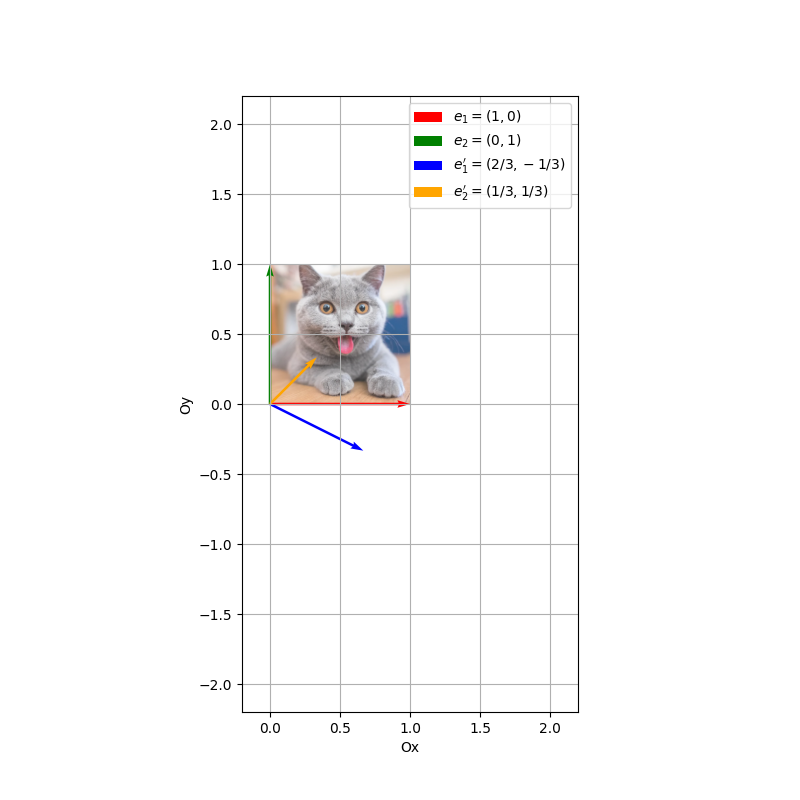
\includegraphics[width=0.45\textwidth]{Images/cat_plot_3.png}
    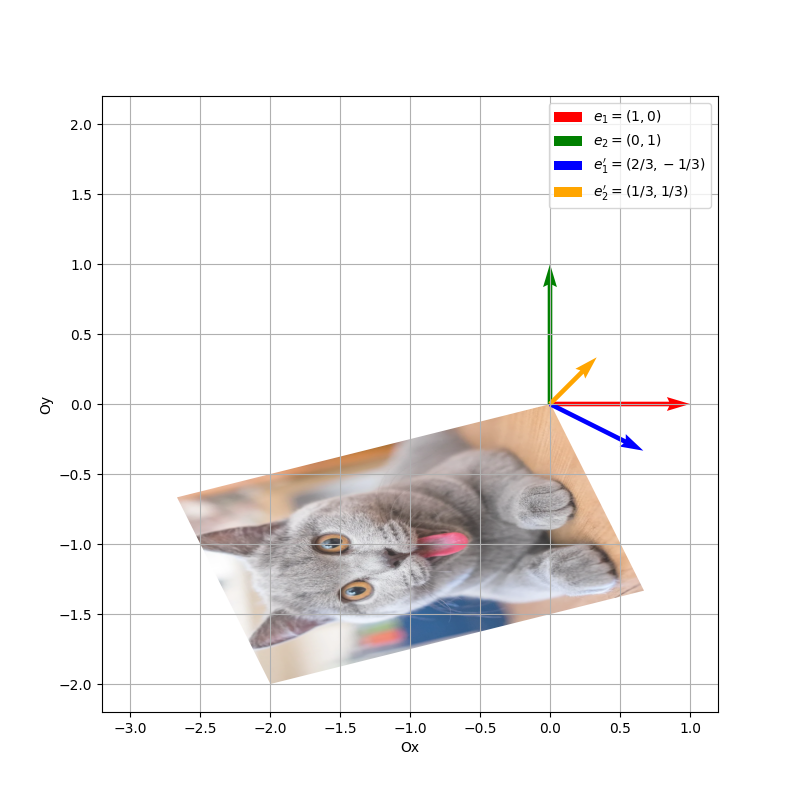
\includegraphics[width=0.45\textwidth]{Images/cat_plot_4.png}
\end{center}

If for any linear operator we could find a basis in which it simply stretches the basis vectors (or reflects and stretches), that would be ideal. Unfortunately, such a basis does not exist for every linear operator, but we will try to get as close to this as possible.
\end{example}

\subsection{Definition of eigenvalues and eigenvectors}

\begin{definition}
Let $T\colon V \to V$ be a linear operator on a vector space $V$ over a field $\F$. A scalar $\lambda \in \F$ is called an \underline{\it eigenvalue} of $T$ if there exists a {\bf nonzero} vector $v \in V$ such that $T(v) = \lambda v$.
The vector $v$ is called an \underline{\it eigenvector} of $T$ corresponding to the eigenvalue $\lambda$.
\end{definition}

\begin{remark}
The zero vector is never considered an eigenvector, even though $T(\mathbf{0}) = \lambda \mathbf{0}$ for any $\lambda$.
\end{remark}

\begin{exercise}
Find eigenvalues and eigenvectors in Example \ref{kitten_transform}.
\end{exercise}

\begin{definition}
Let $\A$ be a linear operator on a finite-dimensional vector space $V$ over a field $\F$. Then the polynomial $\chi_{\A}(t) = \det(t I - \A)\in \F[t]$ is called the \underline{\it characteristic polynomial} of $\A$.
\end{definition}

Since the determinant of a linear operator is basis-independent, the characteristic polynomial is well-defined and can be computed from any matrix of the operator (in any basis).

\begin{example}
Find the characteristic polynomial of the following operators:
\begin{enumerate}
    \item zero operator on $\R^n$,
    \item identity operator on $\R^n$,
    \item operators from Example \ref{kitten_transform},
    \item projection operator on $\R^n$.
\end{enumerate}
\end{example}

If $\dim(V) = n$, then $\deg\chi_{\A}(t) = n$. Consider the coefficients of the characteristic polynomial. The leading coefficient is $1$; the constant term is $\chi_{\A}(0) = \det(-\A) = (-1)^n\det(\A)$.

\begin{exercise}
Find the coefficient of $t^{n-1}$ in the characteristic polynomial of a linear operator.
\end{exercise}

\begin{lemma}
The eigenvalues of a linear operator are the roots of its characteristic polynomial.
\end{lemma}

\begin{proof}
Let $\lambda$ be an eigenvalue of $\A$. Then there exists a nonzero vector $v \in V$ such that $\A(v) = \lambda v$. Then $(\lambda I - \A)(v) = 0$. It means that $\lambda I - \A$ is a degenerate matrix, so $\det(\lambda I - \A) = 0$. Therefore, $\lambda$ is a root of the characteristic polynomial.

If $\lambda$ is a root of the characteristic polynomial, then $\det(\lambda I - \A) = 0$. It means that $\lambda I - \A$ is a degenerate matrix, so there exists a nonzero vector $v \in V$ such that $(\lambda I - \A)(v) = 0$ ($v$ is a nonzero solution of the homogeneous system of linear equations with coefficient matrix $\lambda I - \A$). Therefore, $\lambda$ is an eigenvalue of $\A$.
\end{proof}

\begin{remark}
Note that the definition of an eigenvalue of a linear operator does not depend on the choice of basis. The same eigenvector may have different coordinates in different bases.
\end{remark}

\begin{exercise}
Prove that if the matrix of an operator in some basis is upper triangular (or lower triangular, or diagonal), then its eigenvalues are exactly the entries on the main diagonal.
\end{exercise}

\subsection{Existence of eigenvalues and eigenvectors}

\begin{lemma}
    Every linear operator on a complex finite-dimensional vector space has an eigenvalue and an eigenvector.
\end{lemma}
    
\begin{proof}
This follows immediately from the fundamental theorem of algebra.
\end{proof}

\begin{example}
{\it Why the complex field is necessary?} Because some polynomials have no roots. Consider a linear operator on $\R^2$ with the matrix
$$
A = \begin{pmatrix}
    0 & 1 \\
    -1 & 0
\end{pmatrix}
$$
The characteristic polynomial of this operator is $t^2 + 1$, which has no real roots. Therefore, this operator has no real eigenvalues and eigenvectors in $\R^2$.
\end{example}

\begin{example}
{\it Why the finite dimension is necessary?} Consider the linear operator $\varphi(p(x)) = xp(x)$ on $\R[x]$. Since for any non-zero polynomial $p(x)$, $\deg\varphi(p(x)) = \deg(p(x)) + 1$, then there are no nonzero polynomials, s. t. $\varphi(p(x)) = cp(x)$, where $c\in \R$.
\end{example}
    
It follows from basic polynomial theory that there are at most $n$ eigenvalues. Over $\C$, counting multiplicities, there are exactly $n$ eigenvalues because the equation $\det(tI - \A) = 0$ has exactly $n$ complex roots.

\subsection{Diagonalizable operators}

If we have found at least one eigenvector, we can already simplify the matrix of a linear operator by zeroing the first column below the top entry.

What comes next? Any vector proportional to an eigenvector is also an eigenvector with the same eigenvalue, so we need to look for other eigenvectors. If we can find $n$ linearly independent eigenvectors, we can form a basis and bring the matrix of the linear operator to diagonal form. To understand when this is guaranteed to be possible, we prove the following lemma.

\begin{lemma}
Eigenvectors corresponding to different eigenvalues are linearly independent.
\end{lemma}

\begin{proof}
Prove this by induction on $k$. One eigenvector is linearly independent, because it is nonzero. Assume that $k-1$ eigenvectors are linearly independent and consider $k$ eigenvectors.

Let $\lambda_1, \lambda_2, \ldots, \lambda_k$ be different eigenvalues of $\A$ and $v_1, v_2, \ldots, v_k$ be corresponding eigenvectors. Then $\A(v_i) = \lambda_i v_i$ for $i = 1, 2, \ldots, k$. Consider the linear combination $c_1 v_1 + c_2 v_2 + \ldots + c_k v_k = 0$. Applying $\A$ to both sides, we get $c_1 \lambda_1 v_1 + c_2 \lambda_2 v_2 + \ldots + c_k \lambda_k v_k = 0$. Subtracting the first equation from the second, we get $c_2 (\lambda_2 - \lambda_1) v_2 + \ldots + c_k (\lambda_k - \lambda_1) v_k = 0$. Since $\lambda_i \neq \lambda_j$ for $i \neq j$ and $k-1$ eigenvectors are linearly independent, we have $c_2 = 0, \ldots, c_k = 0$. Therefore, $c_1 = 0$ and the eigenvectors are linearly independent.
\end{proof}

\begin{corollary}
If an operator has $n$ different eigenvalues, then it is diagonalizable in some basis (for example, in the basis of eigenvectors).
\end{corollary}

Note that even if a linear operator has fewer than $n$ distinct eigenvalues, if we happen to find $n$ linearly independent eigenvectors then the operator is diagonalizable in the basis of its eigenvectors.

\subsection{Problems}

\begin{problem}
Find the eigenvalues and eigenvectors of the differentiation operator on $\R_n[x]$.
\end{problem}

\begin{problem}
Find the eigenvalues and eigenvectors of the linear operators given, in some basis, by the following matrices:
\begin{multicols}{2}
\begin{enumerate}[a) ]
\item $\begin{pmatrix}2 & -1 & 2 \\ 5 & -3 & 3 \\ -1 & 0 & -2\end{pmatrix}$,
\item $\begin{pmatrix}0 & 1 & 0 \\ -4 & 4 & 0 \\ -2 & 1 & 2\end{pmatrix}$,
\item $\begin{pmatrix}4 & -5 & 2 \\ 5 & -7 & 3 \\ 6 & -9 & 4\end{pmatrix}$,
\item $\begin{pmatrix}7 & -12 & 6 \\ 10 & -19 & 10 \\ 12 & -24 & 13\end{pmatrix}$,
\item $\begin{pmatrix}4 & -5 & 7 \\ 1 & -4 & 9 \\ -4 & 0 & 5\end{pmatrix}$,
\item $\begin{pmatrix}3 & -1 & 0 & 0 \\ 1 & 1 & 0 & 0 \\ 3 & 0 & 5 & -3 \\ 4 & -1 & 3 & -1\end{pmatrix}$.
\end{enumerate}
\end{multicols}
\end{problem}

\begin{problem}
Find the eigenvalues and eigenvectors of the operators given, in some basis, by the following matrices. Can these operators be diagonalized? If yes, find a corresponding basis and write the change-of-basis matrix and the resulting diagonal matrix.
\begin{multicols}{2}
\begin{enumerate}[a) ]
\item $\begin{pmatrix}0 & 1 \\ 1 & 0\end{pmatrix}$,
\item $\begin{pmatrix}0.5 & 0.5 \\ 0.5 & 0.5\end{pmatrix}$,
\item $\begin{pmatrix}1 & 2 & 3 & 4 \\ 0 & 1 & 2 & 3 \\ 0 & 0 & 1 & 2 \\ 0 & 0 & 0 & 1\end{pmatrix}$,
\item $\begin{pmatrix}2 & 1 & 0 & 0 \\ 0 & 2 & 1 & 0 \\ 0 & 0 & 2 & 1 \\ 0 & 0 & 0 & 2\end{pmatrix}$,
\item $\begin{pmatrix}-1 & 3 & -1 \\ -3 & 5 & -1 \\ -3 & 3 & 1\end{pmatrix}$,
\item $\begin{pmatrix}4 & 7 & -5 \\ -4 & 5 & 0 \\ 1 & 9 & -4\end{pmatrix}$,
\item $\begin{pmatrix}4 & 2 & -5 \\ 6 & 4 & -9 \\ 5 & 3 & -7\end{pmatrix}$,
\item $\begin{pmatrix}1 & 1 & 1 & 1 \\ 1 & 1 & -1 & -1 \\ 1 & -1 & 1 & -1 \\ 1 & -1 & -1 & 1\end{pmatrix}$.
\end{enumerate}
\end{multicols}
\end{problem}

\begin{problem}
Prove and apply basic relations between eigenvalues, determinant, and trace:
\begin{enumerate}[a) ]
\item Prove that for a $2\times 2$ matrix, the product of its eigenvalues equals the determinant of the matrix, and their sum equals the trace.
\item Without computing the characteristic polynomial, find the eigenvalues of the matrix
$$\begin{pmatrix}1 & 2\\ 2 & 1\end{pmatrix}.$$
\end{enumerate}
\end{problem}

\begin{problem}
Compute $A^{100}$ for each matrix:
\begin{enumerate}[a) ]
\item $\begin{pmatrix}1 & 2\\ 2 & 1\end{pmatrix}$,
\item $\begin{pmatrix}7 & -4\\ 14 & -8\end{pmatrix}$,
\item $\begin{pmatrix}1 & -3 & 4 \\ 4 & -7 & 8 \\ 6 & -7 & 7\end{pmatrix}$,
\item $\begin{pmatrix}4 & -5 & 7 \\ 1 & -4 & 9 \\ -4 & 0 & 5\end{pmatrix}$,
\item $\begin{pmatrix}1 & -2 \\ 1 & -1\end{pmatrix}$.
\end{enumerate}
\end{problem}

\begin{problem}
Find a closed formula for the $n$-th Fibonacci number. Recall that the Fibonacci numbers are defined by
$$
F_0 = 0, \quad F_1 = 1, \quad F_n = F_{n-1} + F_{n-2} \quad \text{for } n \geq 2.
$$
\end{problem}

\begin{problem}
Find $A^n$ for any natural number $n$ for the matrix 
$$
A = \begin{pmatrix}
    1 & 0 & 0 \\
    2 & 1 & -1\\
    1 & 3 & -2
\end{pmatrix}.
$$
\end{problem}
% char polynomial: $t^3 - 1$.

\begin{problem}
Find a closed formula for the solution of the following recurrence relations:
\begin{enumerate}[a) ]
\item $u(n)=3 u(n-1)-2 u(n-2), \quad u(0)=-2, \quad u(1)=1$;
\item $u(n)=-2 u(n-1)-u(n-2), \quad u(0)=-1, \quad u(1)=-1$.
\end{enumerate}
\end{problem}